\documentclass[]{article}
\usepackage{amssymb,amsmath}
\usepackage{ifxetex,ifluatex}
\ifxetex
  \usepackage{fontspec,xltxtra,xunicode}
  \defaultfontfeatures{Mapping=tex-text,Scale=MatchLowercase}
  \newcommand{\euro}{€}
\else
  \ifluatex
    \usepackage{fontspec}
    \defaultfontfeatures{Mapping=tex-text,Scale=MatchLowercase}
    \newcommand{\euro}{€}
  \else
    \usepackage[utf8]{inputenc}
    \usepackage{eurosym}
  \fi
\fi
\usepackage{color}
\usepackage{fancyvrb}
\DefineShortVerb[commandchars=\\\{\}]{\|}
\DefineVerbatimEnvironment{Highlighting}{Verbatim}{commandchars=\\\{\}}
% Add ',fontsize=\small' for more characters per line
\newenvironment{Shaded}{}{}
\newcommand{\KeywordTok}[1]{\textcolor[rgb]{0.00,0.44,0.13}{\textbf{{#1}}}}
\newcommand{\DataTypeTok}[1]{\textcolor[rgb]{0.56,0.13,0.00}{{#1}}}
\newcommand{\DecValTok}[1]{\textcolor[rgb]{0.25,0.63,0.44}{{#1}}}
\newcommand{\BaseNTok}[1]{\textcolor[rgb]{0.25,0.63,0.44}{{#1}}}
\newcommand{\FloatTok}[1]{\textcolor[rgb]{0.25,0.63,0.44}{{#1}}}
\newcommand{\CharTok}[1]{\textcolor[rgb]{0.25,0.44,0.63}{{#1}}}
\newcommand{\StringTok}[1]{\textcolor[rgb]{0.25,0.44,0.63}{{#1}}}
\newcommand{\CommentTok}[1]{\textcolor[rgb]{0.38,0.63,0.69}{\textit{{#1}}}}
\newcommand{\OtherTok}[1]{\textcolor[rgb]{0.00,0.44,0.13}{{#1}}}
\newcommand{\AlertTok}[1]{\textcolor[rgb]{1.00,0.00,0.00}{\textbf{{#1}}}}
\newcommand{\FunctionTok}[1]{\textcolor[rgb]{0.02,0.16,0.49}{{#1}}}
\newcommand{\RegionMarkerTok}[1]{{#1}}
\newcommand{\ErrorTok}[1]{\textcolor[rgb]{1.00,0.00,0.00}{\textbf{{#1}}}}
\newcommand{\NormalTok}[1]{{#1}}
% Redefine labelwidth for lists; otherwise, the enumerate package will cause
% markers to extend beyond the left margin.
\makeatletter\AtBeginDocument{%
  \renewcommand{\@listi}
    {\setlength{\labelwidth}{4em}}
}\makeatother
\usepackage{enumerate}
\usepackage{ctable}
\usepackage{float} % provides the H option for float placement
\usepackage{graphicx}
% We will generate all images so they have a width \maxwidth. This means
% that they will get their normal width if they fit onto the page, but
% are scaled down if they would overflow the margins.
\makeatletter
\def\maxwidth{\ifdim\Gin@nat@width>\linewidth\linewidth
\else\Gin@nat@width\fi}
\makeatother
\let\Oldincludegraphics\includegraphics
\renewcommand{\includegraphics}[1]{\Oldincludegraphics[width=\maxwidth]{#1}}
\ifxetex
  \usepackage[setpagesize=false, % page size defined by xetex
              unicode=false, % unicode breaks when used with xetex
              xetex,
              colorlinks=true,
              linkcolor=blue]{hyperref}
\else
  \usepackage[unicode=true,
              colorlinks=true,
              linkcolor=blue]{hyperref}
\fi
\hypersetup{breaklinks=true, pdfborder={0 0 0}}
\setlength{\parindent}{0pt}
\setlength{\parskip}{6pt plus 2pt minus 1pt}
\setlength{\emergencystretch}{3em}  % prevent overfull lines
\usepackage[top=2cm,bottom=2cm,left=2cm,right=2cm,a4paper]{geometry}
\usepackage[frenchb]{babel}
%\usepackage{lscape}
%\usepackage{color}
%\definecolor{vert}{rgb}{0,0.5,0}
%\definecolor{bleu}{rgb}{0,0,0.5}
%\lstset{language=Python,basicstyle=\ttfamily\footnotesize,commentstyle=\color{vert},keywordstyle=\color{bleu}}

\title{Langages de balisage légers et logiciels de conversion de documents}
\author{Nicolas Poulain}

\begin{document}
\maketitle

\section{Présentation}

Pour saisir et mettre en forme des textes ou des documents textuels
comportant des insertions d'images, de figures ou de tableaux, on
utilise généralement un traitement de texte WYSIWYG\footnote{Un WYSIWYG
  pour \emph{What you see is what you get} est une interface utilisateur
  qui permet de composer visuellement le résultat voulu. C'est une
  interface intuitive : l'utilisateur voit directement à l'écran à quoi
  ressemblera le résultat final.}, propriétaire comme Microsoft Word ou
libre comme OpenOffice.

Les défauts majeurs de ces logiciels sont nombreux :

\begin{enumerate}[1.]
\item
  Le rédacteur d'un document se concentre presque autant autant sur le
  fond que sur la forme. Outre le temps passé, les conséquences sur le
  rendu sont nombreuses
  \begin{itemize}
  \item
    Les mises en forme les plus hétéroclites sont autorisées au dépens
    de la lisibilité ;
  \item
    Le résultat final est souvent discutable du point du vue de la
    typographie car les règles n'en sont pas respectées ni par
    l'utilisateur ni par le logiciel ;
  \item
    L'utilisation des styles est souvent anarchique et les documents mal
    structurés, ce qui rend la production automatique de sommaire ou
    d'index impossible ;
  \item
    L'insertion d'images ou de figures provoque des décalages mal
    maîtrisés.
  \end{itemize}
\item
  En ce qui concerne les documents longs, l'inclusion de documents
  annexes au sein du document maître donne des résultats aléatoires ;
\item
  L'interopérabilité n'est pas assurée entre les logiciels, elle ne
  l'est pas même entre les différentes versions d'un même logiciel, ce
  qui nous amène au dernier point ;
\item
  La pérénnité des documents n'est pas certaine puisque la compatibilité
  ascendante ne fonctionne pas toujours et qu'un document écrit il y a
  quelques années risque d'être perdu, faute du logiciel capable de le
  lire.
\end{enumerate}
À l'opposé de la composition dans un logiciel de traitement de texte, on
peut écrire des documents dans des langages de balisage. Il en existe de
nombreux : LaTeX, HTML, DocBook, etc. Les fichiers sont enregistrés au
format texte brut et doivent être interprétés par un logiciel afin
d'être consultés.

En ce qui concerne HTML et LaTeX, où pratiquement toutes les mises en
formes sont possibles, le problème vient de la difficulté à écrire les
balises\footnote{Dans le cas du format DocBook, c'est même humainement
  presque impossible de l'écrire à la main tant l'enchevêtrement des
  balises est inextriquable. On le génère avec un logiciel
  WYSIWYG\ldots{}}. Pour écrire un titre suivi d'une phrase contenant un
mot en gras puis une liste non numérotée, on saisira respecivement :

\begin{itemize}
\item
  en LaTeX

\begin{verbatim}
    \section{Le titre du paragraphe}

    Voici un mot en \textbf{gras} puis une liste :

    \begin{enumerate}
     \item  c'est simple ;
     \item  c'est efficace.
    \end{enumerate}
\end{verbatim}
\item
  en HTML

\begin{verbatim}
    <h1>Le titre du paragraphe</h1>
    <p>Voici un mot en <strong>gras</strong> puis une liste :</p>
    <ul>
     <li> c'est simple ;</li>
     <li> c'est efficace.</li>
    </ul>
\end{verbatim}
\end{itemize}
Comme on le voit, la syntaxe est accessible mais au goût de nombreux
utilisateurs il y a trop de commandes de mise en forme qui nuisent à la
lisibilité du texte lors de la saisie. C'est dommage car ces deux
formats ouverts et universels ont chacun leur avantage :

\begin{itemize}
\item
  HTML peut être lu sur n'importe quelle plateforme ou terminal du monde
  entier car ses spécifications, gérées le W3C\footnote{Un WYSIWYG pour
    \emph{What you see is what you get} est une interface utilisateur
    qui permet de composer visuellement le résultat voulu. C'est une
    interface intuitive : l'utilisateur voit directement à l'écran à
    quoi ressemblera le résultat final.}, sont respectées par les
  navigateurs web.
\item
  le logiciel LaTeX produit des documents de qualité unanimement
  reconnue. Il prend en charge la mise en page, l'utilisateur n'ayant
  qu'à se concentrer sur le fond et sa structure.
\end{itemize}
Il existe une alternative qui est à la fois simple, interopérable et
efficace : les langages de balisage légers.

\section{Les langages de balisage légers et les wikis}

Un langage de balisage léger est un langage utilisant une syntaxe
simple, conçue pour qu'un fichier en ce langage soit aisé à saisir avec
un éditeur de texte simple, et facile à lire dans sa forme non formatée.

Les wikis on grandement contribué à populariser ce type de langage. Le
principe est de saisir des balises accessibles aux non inités, un moteur
se chargeant de la conversion en HTML avant la publication.

\begin{verbatim}
Le titre du paragraphe
======================

Voici un mot en **gras** puis une liste :

* c'est simple ;
* c'est efficace.
\end{verbatim}
Avantages :

\begin{itemize}
\item
  les balises sont visuelles et le texte reste lisible ;
\item
  le nombre de balises et de règles est très limité donc
  \begin{itemize}
  \item
    la syntaxe est facile à mémoriser ;
  \item
    il est relativement simple de programmer un logiciel capable
    d'interpréter un de ces langages
  \end{itemize}
\item
  les balises étant constituées de cractères non alphabétiques, on peut
  utiliser un correcteur d'othographe.
\end{itemize}
Il existe de nombreux langages de balisage légers : Creole, Markdown,
Asciidoc, etc. Chacun a ses avantages, mais tous sont simples.

Dans la section suivante, nous allons voir qu'il est possible faire de
la bureautique avec ces langages et nous verrons lequel choisir en
fonction de l'usage qu'on souhaite en faire.

\section{Les langages de balisage légers et la bureautique}

On vient de voir qu'au sein des wikis, les langages de balisage légers
sont transformés en HTML.

C'est maintenant que les choses deviennent intéressantes : il existe des
logiciels permettant d'exporter et de mettre en forme vers différents
formats pour différents usages : la diffusion web, bien sûr mais aussi
l'export pour un traitement de texte, l'impression, la lecture sur
tablette ou liseuse d'e-book ou encore la vidéo-projection.

Ces logiciels de conversion sont nombreux, en voici trois avec leurs
principaux formats d'import et d'export.

\ctable[pos = H, center, botcap]{llllll}
{% notes
}
{% rows
\FL
\parbox[b]{0.14\columnwidth}{\raggedright
Logiciel
} & \parbox[b]{0.14\columnwidth}{\raggedright
Import
} & \parbox[b]{0.13\columnwidth}{\raggedright
Export web
} & \parbox[b]{0.18\columnwidth}{\raggedright
Export Bureautique
} & \parbox[b]{0.13\columnwidth}{\raggedright
Export TeX
} & \parbox[b]{0.13\columnwidth}{\raggedright
Export LBL
}
\ML
\parbox[t]{0.14\columnwidth}{\raggedright
Txt2tags
} & \parbox[t]{0.14\columnwidth}{\raggedright
T2t
} & \parbox[t]{0.13\columnwidth}{\raggedright
HTML, XHTML, SGML,
} & \parbox[t]{0.18\columnwidth}{\raggedright
DocBook, Lout, MagicPoint, PageMaker
} & \parbox[t]{0.13\columnwidth}{\raggedright
LaTeX
} & \parbox[t]{0.13\columnwidth}{\raggedright
Creole, AsciiDoc, PmWiki, MoinMoin, AsciiDoc, DokuWiki
}
\\\noalign{\medskip}
\parbox[t]{0.14\columnwidth}{\raggedright
Pandoc
} & \parbox[t]{0.14\columnwidth}{\raggedright
Markdown, LaTeX, HTML, Textile, RST
} & \parbox[t]{0.13\columnwidth}{\raggedright
HTML, XHTML, HTML5, EPUB, Slidy,S5, DZSlides
} & \parbox[t]{0.18\columnwidth}{\raggedright
OpenDocument, ODT, DOCX, DocBook
} & \parbox[t]{0.13\columnwidth}{\raggedright
LaTeX, ConTeXt, Beamer
} & \parbox[t]{0.13\columnwidth}{\raggedright
Markdown, RST, AsciiDoc, Textile, MediaWiki
}
\\\noalign{\medskip}
\parbox[t]{0.14\columnwidth}{\raggedright
AsciiDoc
} & \parbox[t]{0.14\columnwidth}{\raggedright
AsciiDoc
} & \parbox[t]{0.13\columnwidth}{\raggedright
HTML, XHTML
} & \parbox[t]{0.18\columnwidth}{\raggedright
Docbook
} & \parbox[t]{0.13\columnwidth}{\raggedright
LaTeX
} & \parbox[t]{0.13\columnwidth}{\raggedright
}
\LL
}

\ctable[pos = H, center, botcap]{llll}
{% notes
}
{% rows
\FL
\parbox[b]{0.43\columnwidth}{\raggedright
Fonctionnalités
} & \parbox[b]{0.13\columnwidth}{\raggedright
Txt2tags
} & \parbox[b]{0.10\columnwidth}{\raggedright
Pandoc
} & \parbox[b]{0.10\columnwidth}{\raggedright
Asciidoc
}
\ML
\parbox[t]{0.43\columnwidth}{\raggedright
en-tête (titre, auteur, date)
} & \parbox[t]{0.13\columnwidth}{\raggedright
x
} & \parbox[t]{0.10\columnwidth}{\raggedright
x
} & \parbox[t]{0.10\columnwidth}{\raggedright
x
}
\\\noalign{\medskip}
\parbox[t]{0.43\columnwidth}{\raggedright
sections (numérotées ou non)
} & \parbox[t]{0.13\columnwidth}{\raggedright
x
} & \parbox[t]{0.10\columnwidth}{\raggedright
x
} & \parbox[t]{0.10\columnwidth}{\raggedright
x
}
\\\noalign{\medskip}
\parbox[t]{0.43\columnwidth}{\raggedright
paragraphes
} & \parbox[t]{0.13\columnwidth}{\raggedright
x
} & \parbox[t]{0.10\columnwidth}{\raggedright
x
} & \parbox[t]{0.10\columnwidth}{\raggedright
x
}
\\\noalign{\medskip}
\parbox[t]{0.43\columnwidth}{\raggedright
listes à puces, numérotées et de définition
} & \parbox[t]{0.13\columnwidth}{\raggedright
x
} & \parbox[t]{0.10\columnwidth}{\raggedright
x
} & \parbox[t]{0.10\columnwidth}{\raggedright
x
}
\\\noalign{\medskip}
\parbox[t]{0.43\columnwidth}{\raggedright
texte en gras, italique, souligné, barré
} & \parbox[t]{0.13\columnwidth}{\raggedright
x
} & \parbox[t]{0.10\columnwidth}{\raggedright
x
} & \parbox[t]{0.10\columnwidth}{\raggedright
x
}
\\\noalign{\medskip}
\parbox[t]{0.43\columnwidth}{\raggedright
couleurs et tailles de texte
} & \parbox[t]{0.13\columnwidth}{\raggedright
} & \parbox[t]{0.10\columnwidth}{\raggedright
} & \parbox[t]{0.10\columnwidth}{\raggedright
x
}
\\\noalign{\medskip}
\parbox[t]{0.43\columnwidth}{\raggedright
police à espacement constant
} & \parbox[t]{0.13\columnwidth}{\raggedright
x
} & \parbox[t]{0.10\columnwidth}{\raggedright
x
} & \parbox[t]{0.10\columnwidth}{\raggedright
x
}
\\\noalign{\medskip}
\parbox[t]{0.43\columnwidth}{\raggedright
coloration syntaxique de code source
} & \parbox[t]{0.13\columnwidth}{\raggedright
} & \parbox[t]{0.10\columnwidth}{\raggedright
x
} & \parbox[t]{0.10\columnwidth}{\raggedright
x
}
\\\noalign{\medskip}
\parbox[t]{0.43\columnwidth}{\raggedright
gestion des liens (internet, courriel, etc.)
} & \parbox[t]{0.13\columnwidth}{\raggedright
x
} & \parbox[t]{0.10\columnwidth}{\raggedright
x
} & \parbox[t]{0.10\columnwidth}{\raggedright
x
}
\\\noalign{\medskip}
\parbox[t]{0.43\columnwidth}{\raggedright
Références internes
} & \parbox[t]{0.13\columnwidth}{\raggedright
} & \parbox[t]{0.10\columnwidth}{\raggedright
x
} & \parbox[t]{0.10\columnwidth}{\raggedright
x
}
\\\noalign{\medskip}
\parbox[t]{0.43\columnwidth}{\raggedright
images
} & \parbox[t]{0.13\columnwidth}{\raggedright
x
} & \parbox[t]{0.10\columnwidth}{\raggedright
x
} & \parbox[t]{0.10\columnwidth}{\raggedright
x
}
\\\noalign{\medskip}
\parbox[t]{0.43\columnwidth}{\raggedright
tableaux (gestion de bordure et d'alignement)
} & \parbox[t]{0.13\columnwidth}{\raggedright
x
} & \parbox[t]{0.10\columnwidth}{\raggedright
x
} & \parbox[t]{0.10\columnwidth}{\raggedright
x
}
\\\noalign{\medskip}
\parbox[t]{0.43\columnwidth}{\raggedright
tableaux (fusion de cellules)
} & \parbox[t]{0.13\columnwidth}{\raggedright
} & \parbox[t]{0.10\columnwidth}{\raggedright
} & \parbox[t]{0.10\columnwidth}{\raggedright
x
}
\\\noalign{\medskip}
\parbox[t]{0.43\columnwidth}{\raggedright
Légendes (images et tableaux)
} & \parbox[t]{0.13\columnwidth}{\raggedright
} & \parbox[t]{0.10\columnwidth}{\raggedright
x
} & \parbox[t]{0.10\columnwidth}{\raggedright
x
}
\\\noalign{\medskip}
\parbox[t]{0.43\columnwidth}{\raggedright
Citations
} & \parbox[t]{0.13\columnwidth}{\raggedright
} & \parbox[t]{0.10\columnwidth}{\raggedright
x
} & \parbox[t]{0.10\columnwidth}{\raggedright
x
}
\\\noalign{\medskip}
\parbox[t]{0.43\columnwidth}{\raggedright
Notes de bas de page
} & \parbox[t]{0.13\columnwidth}{\raggedright
} & \parbox[t]{0.10\columnwidth}{\raggedright
x
} & \parbox[t]{0.10\columnwidth}{\raggedright
x
}
\\\noalign{\medskip}
\parbox[t]{0.43\columnwidth}{\raggedright
formules mathématiques (LaTeX)
} & \parbox[t]{0.13\columnwidth}{\raggedright
} & \parbox[t]{0.10\columnwidth}{\raggedright
x
} & \parbox[t]{0.10\columnwidth}{\raggedright
x
}
\LL
}

Comme on le voit, ces outils ne sont pas conçus pour permettre de
changer de police, obtenir des effets de couleur, etc.

\begin{figure}[htbp]
\centering

\includegraphics{degrade.png}
\caption{A-t-on vraiment besoin de ceci ?}
\end{figure}

\section{Comment s'y prendre concrètement}

Maintenant que l'environnement est décrit, étudions des exemples.

\subsection{Un document essentiellement textuel}

Comme le document est simple, nous utilisons ici le lociciel txt2tags
dont la syntaxe est entièrement décrite sur la page
http://txt2tags.org/markup.html

Voici le document à rédiger.

\begin{figure}[htbp]
\centering
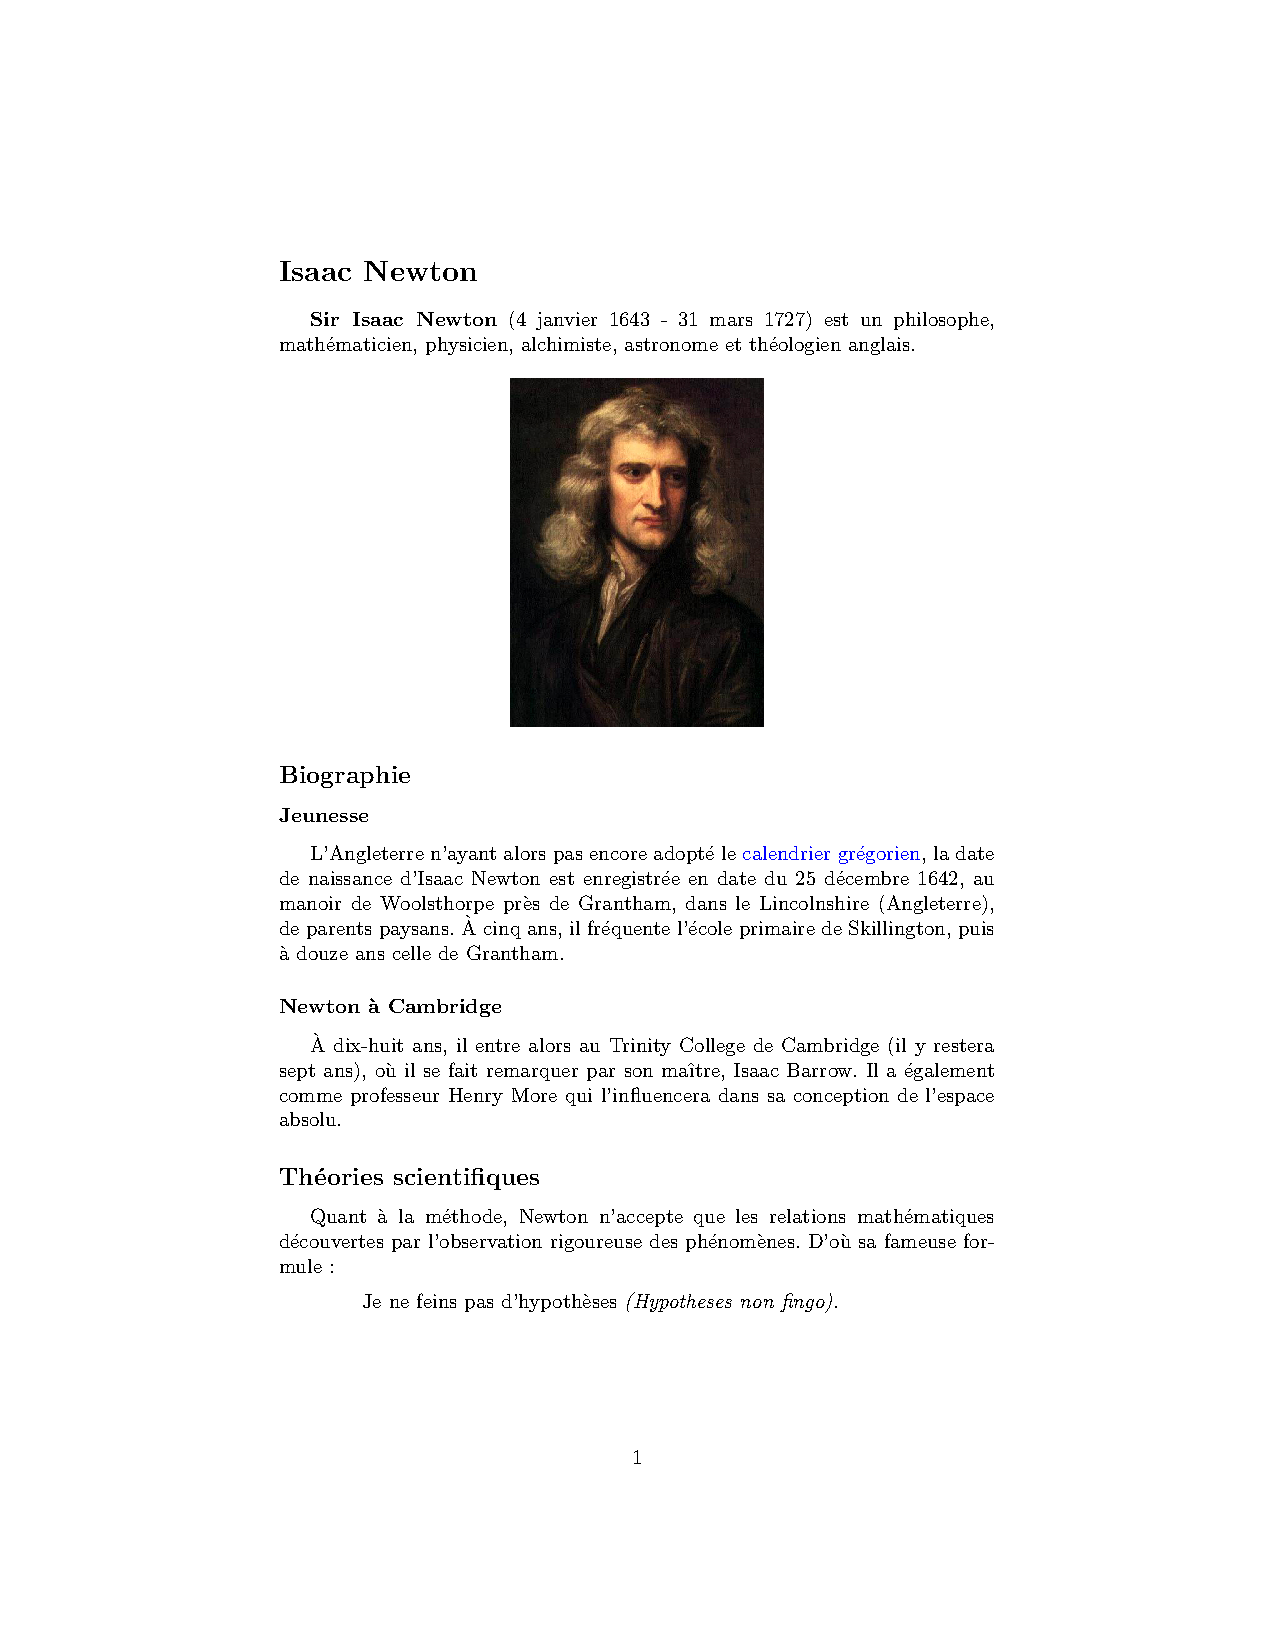
\includegraphics{newton.pdf}
\caption{Un document produit par txt2tags}
\end{figure}

\begin{verbatim}
    Fiche sur Isaac Newton 
    D'après wikipédia
    Lundi 32 Janvier 2029

    = Isaac Newton =

    **Sir Isaac Newton** (4 janvier 1643 - 31 mars 1727) est un philosophe,
    mathématicien, physicien, alchimiste, astronome et théologien anglais.

       | [IsaacNewton.jpg]

    == Biographie ==

    === Jeunesse ===

    L'Angleterre n'ayant alors pas encore adopté le 
    [calendrier grégorien http://fr.wikipedia.org/wiki/Calendrier_gr%C3%A9gorien],
    la date de naissance d’Isaac Newton est enregistrée en date du 25 décembre 1642,
    au manoir de Woolsthorpe près de Grantham, dans le Lincolnshire (Angleterre),
    de parents paysans. 
    À cinq ans, il fréquente l’école primaire de Skillington, puis à
    douze ans celle de Grantham.

    === Newton à Cambridge ===

    À dix-huit ans, il entre alors au Trinity College de Cambridge (il y restera
    sept ans), où il se fait remarquer par son maître, Isaac Barrow. Il a également
    comme professeur Henry More qui l'influencera dans sa conception de l'espace
    absolu.

    == Théories scientifiques ==

    Quant à la méthode, Newton n'accepte que les relations mathématiques découvertes
    par l'observation rigoureuse des phénomènes. D'où sa fameuse formule :
         Je ne feins pas d'hypothèses //(Hypotheses non fingo)//.
\end{verbatim}
Comme on le voit, les tailles des titres sont automatiques, la gestion
des paragraphes ainsi que celle des césures est laissée au logiciel. Le
lien hypertexte a été traduit de même que les changements de style
(gras, italique) ainsi que la citation indentée. Les trois premières
lignes constituent la page de garde (non reproduite ici) du document.

Comment ce document mis en forme a-t-il été produit : Disons que le
texte a été enregistré dans un fichier \texttt{newton.t2t}, alors la
commande suivante va produire le fichier \texttt{newton.pdf}.

\begin{verbatim}
$ txt2tags -t tex newton.t2t && pdflatex newton.tex
\end{verbatim}
Pour obtenir une version html, la commande suivante fonctionne

\begin{verbatim}
$ txt2tags -t html newton.t2t
\end{verbatim}
Conclusion : le logiciel txt2tags avec sa syntaxe simpliste permet de
produire des documents courants de façon très simple.

\subsection{Un document scientifique}

La syntaxe txt2tags vue plus haut est simpliste\footnote{Statut assumé
  par l'auteur qui souhaite rester dans la ligne de l'acronyme KISS
  (\emph{Keep It Simple, Stupid}). Voir
  http://fr.wikipedia.org/wiki/Keep\_it\_Simple,\_Stupid}, cependant
l'export vers le langage de balisage léger nommé Markdown est possible.

Le langage Markdown utilisé par logiciel Pandoc possède des
fonctionnalités supplémentaires comme nous le montre l'exemple suivant.

\begin{figure}[htbp]
\centering
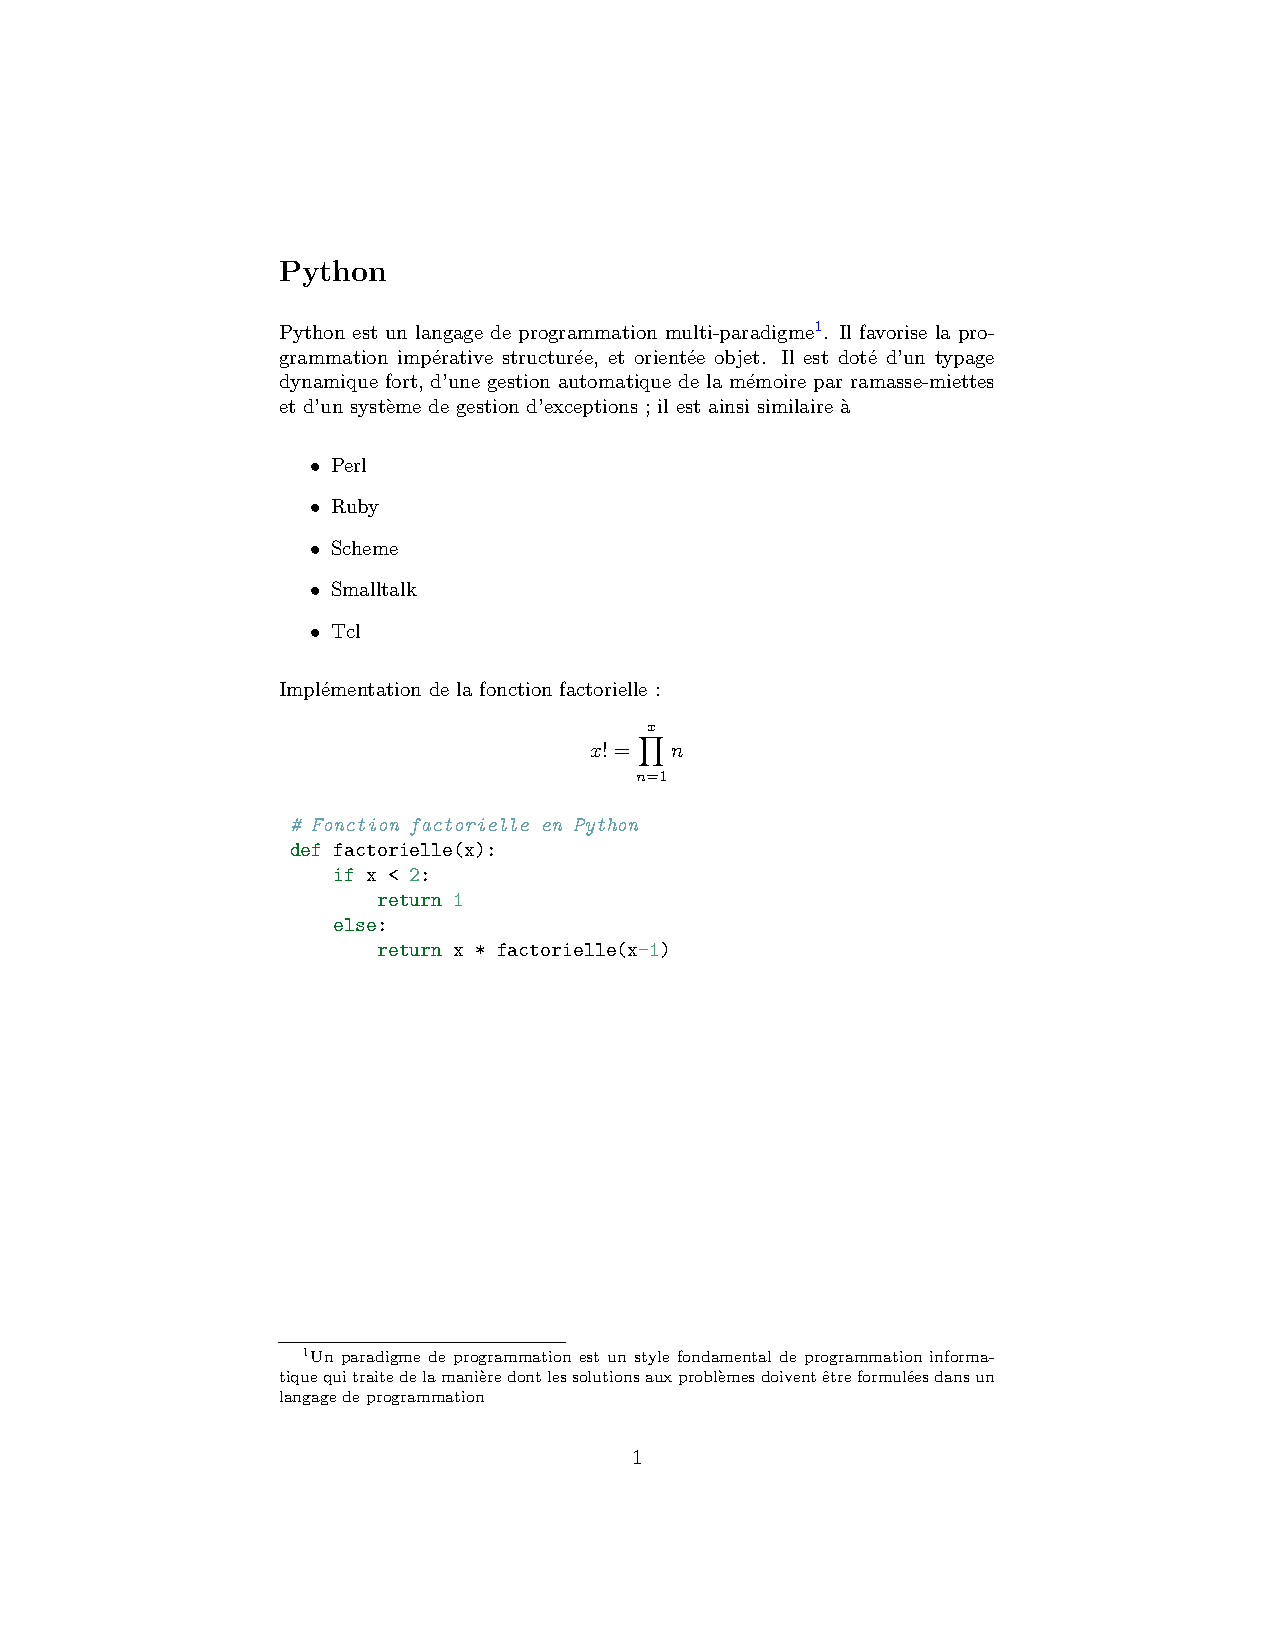
\includegraphics{python.pdf}
\caption{Un document produit par Pandoc}
\end{figure}

\begin{verbatim}

    Python
    ======

    Python est un langage de programmation multi-paradigme[^1]. Il favorise la
    programmation impérative structurée, et orientée objet. Il est doté d'un typage
    dynamique fort, d'une gestion automatique de la mémoire par ramasse-miettes et
    d'un système de gestion d'exceptions ; il est ainsi similaire à 

    * Perl
    * Ruby
    * Scheme
    * Smalltalk
    * Tcl

    [^1]:Un paradigme de programmation est un style fondamental de programmation
    informatique qui traite de la manière dont les solutions aux problèmes doivent
    être formulées dans un langage de programmation

    Implémentation de la fonction factorielle :
    $$ x! = \prod_{n=1}^x n $$

    ```Python
     # Fonction factorielle en Python
     def factorielle(x):
         if x < 2:
         return 1
         else:
         return x * factorielle(x-1)
    ```
\end{verbatim}
Observez l'inserion de la formule mathématique (syntaxe LaTeX) ainsi que
la coloration syntaxique du code source selon le nom du langage choisi.

Comment ce document mis en forme a-t-il été produit ? Disons que le
texte a été enregistré dans un fichier \texttt{python.md}, alors la
commande suivante va produire le fichier \texttt{python.pdf}.

\begin{Shaded}
\begin{Highlighting}[]
\NormalTok{$ pandoc --highlight-style=pygments -s python.md -o python.pdf}
\end{Highlighting}
\end{Shaded}
Pour obtenir une version html, la commande suivante fonctionne

\begin{verbatim}
$ pandoc --highlight-style=pygments -s python.md -o python.html
\end{verbatim}

\end{document}
